% LaTeX figure includes for Vortex-Codec paper
% Include this file in your main document or copy relevant figures

\begin{figure}[htbp]
    \centering
    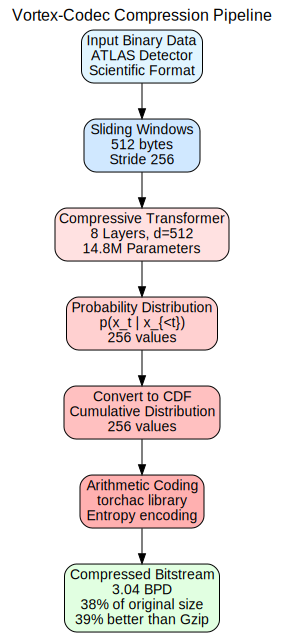
\includegraphics[width=0.9\textwidth]{figures/figure1_compression_pipeline.pdf}
    \caption{Vortex-Codec compression pipeline showing the complete flow from input binary data through the compressive transformer to compressed output.}
    \label{fig:compression_pipeline}
\end{figure}

\begin{figure}[htbp]
    \centering
    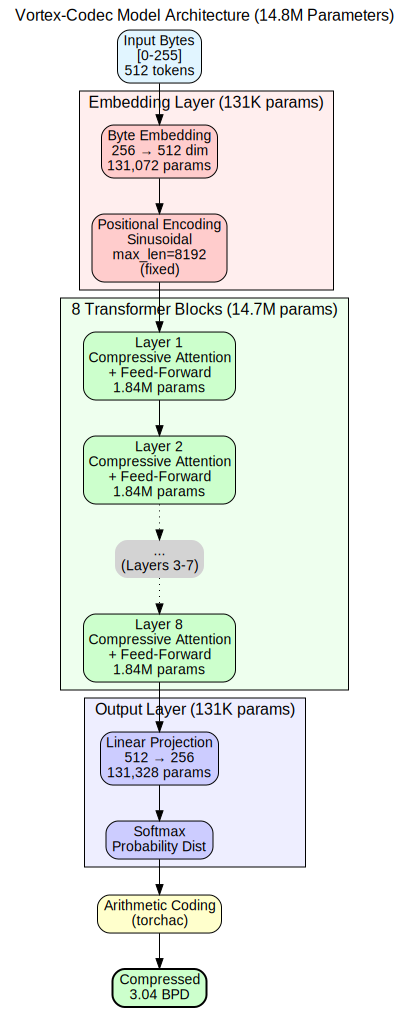
\includegraphics[width=\textwidth]{figures/figure2_model_architecture.pdf}
    \caption{Complete model architecture with 14.8M parameters. The model consists of byte embedding, 8 compressive transformer layers, and output projection.}
    \label{fig:model_architecture}
\end{figure}

\begin{figure}[htbp]
    \centering
    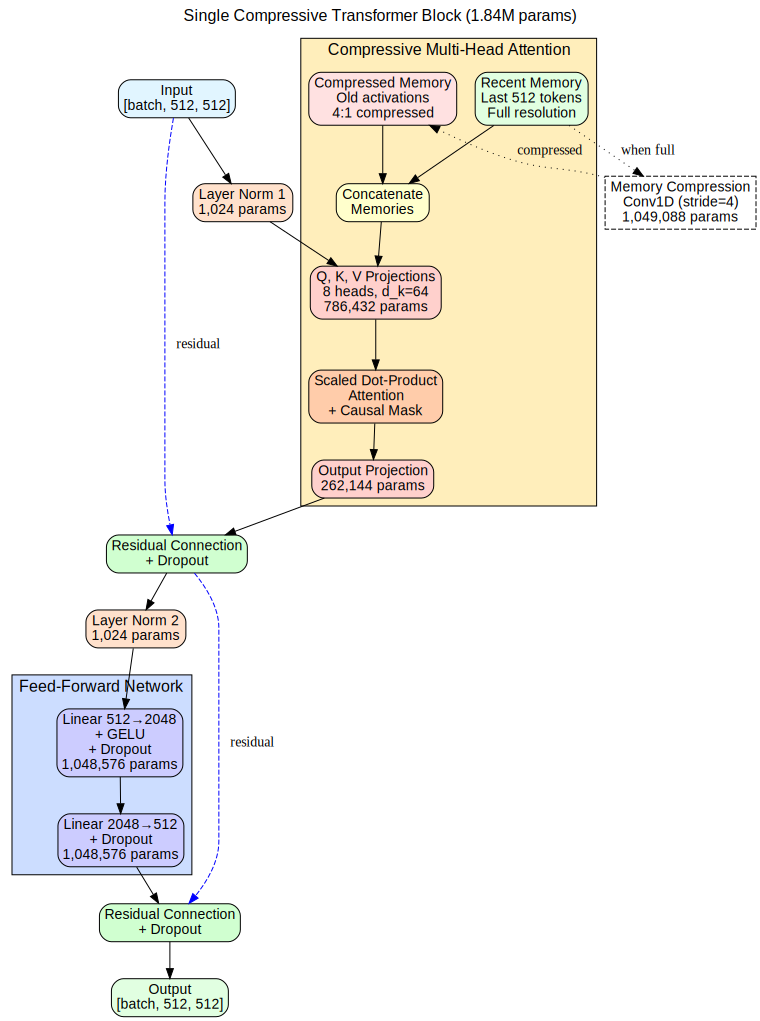
\includegraphics[width=0.95\textwidth]{figures/figure3_transformer_block.pdf}
    \caption{Detailed view of a single compressive transformer block (1.84M parameters) showing compressive attention and feed-forward components.}
    \label{fig:transformer_block}
\end{figure}

\begin{figure}[htbp]
    \centering
    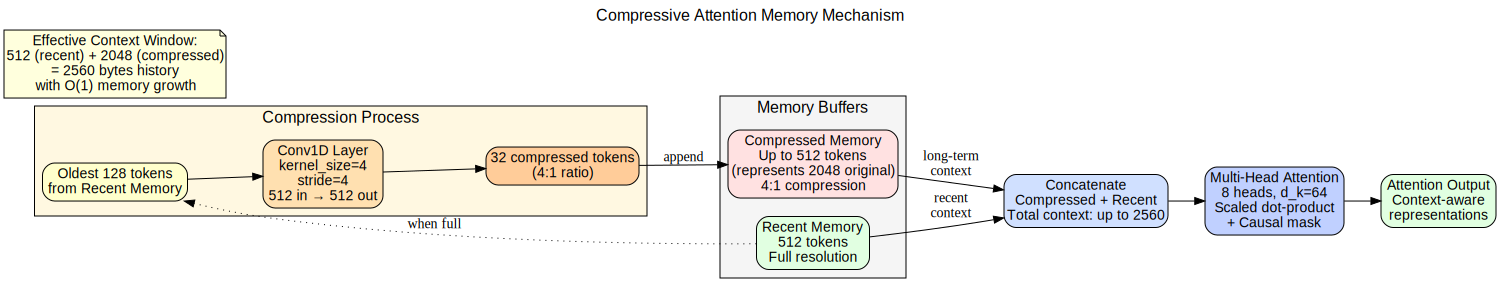
\includegraphics[width=0.9\textwidth]{figures/figure4_compressive_attention.pdf}
    \caption{Compressive attention mechanism with two-tier memory system: recent memory (512 tokens) and compressed memory (4:1 ratio).}
    \label{fig:compressive_attention}
\end{figure}

\begin{figure}[htbp]
    \centering
    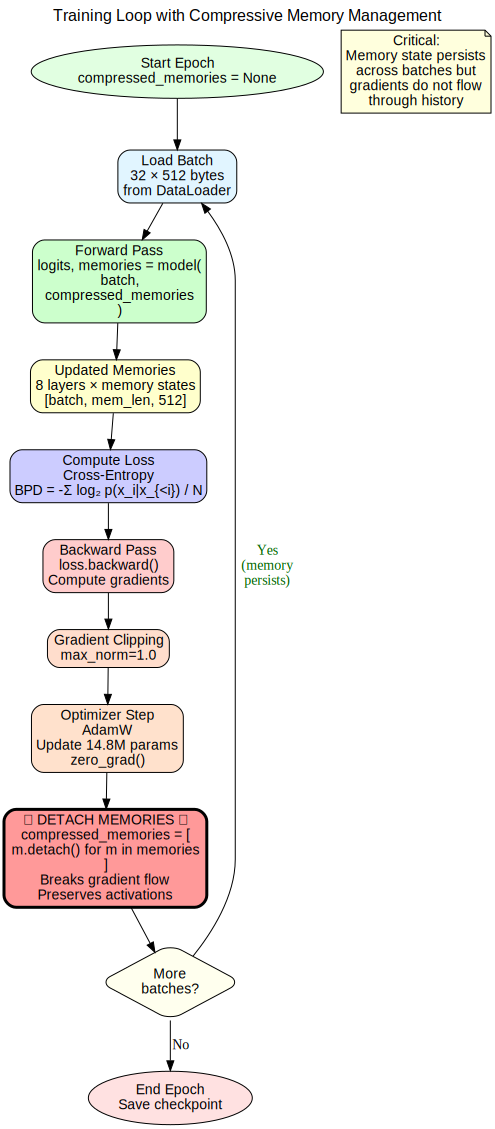
\includegraphics[width=0.8\textwidth]{figures/figure5_training_loop.pdf}
    \caption{Training loop with compressive memory management. The critical memory detachment step prevents gradient flow through sequence history.}
    \label{fig:training_loop}
\end{figure}

\begin{figure}[htbp]
    \centering
    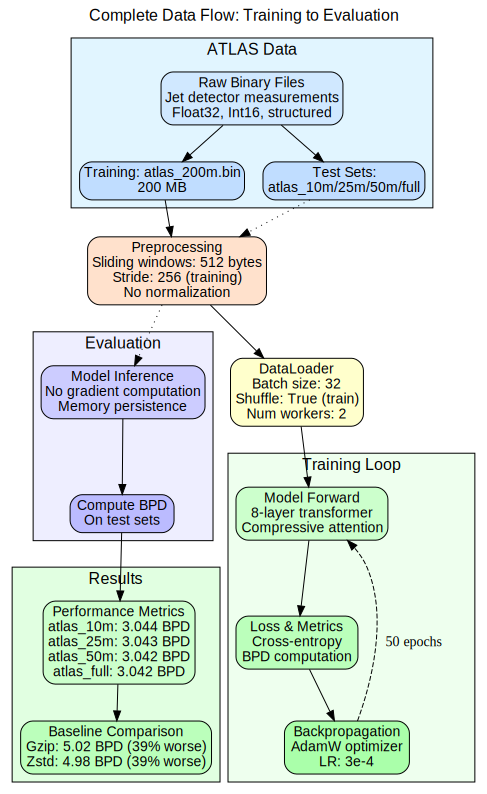
\includegraphics[width=\textwidth]{figures/figure6_data_flow.pdf}
    \caption{Complete data flow from raw ATLAS data through preprocessing, training, and evaluation.}
    \label{fig:data_flow}
\end{figure}

\begin{figure}[htbp]
    \centering
    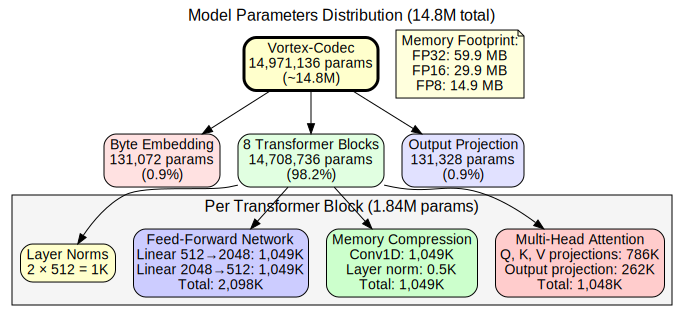
\includegraphics[width=0.8\textwidth]{figures/figure7_parameters.pdf}
    \caption{Parameter distribution across model components. Transformer blocks comprise 98.2\% of the 14.8M total parameters.}
    \label{fig:parameters}
\end{figure}

\begin{figure}[htbp]
    \centering
    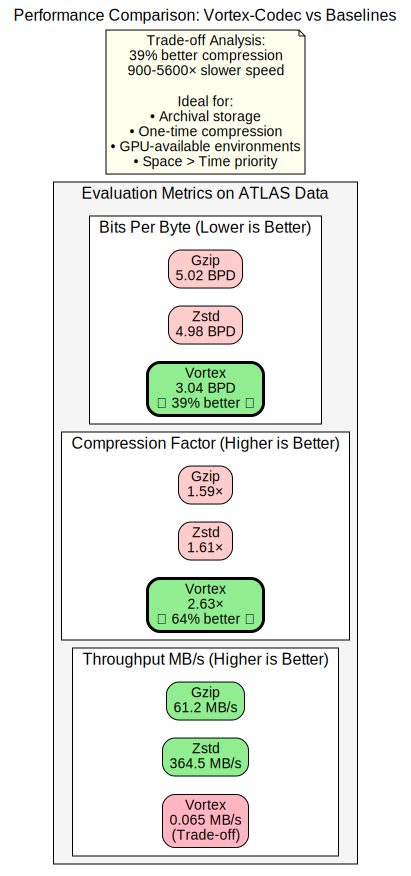
\includegraphics[width=0.9\textwidth]{figures/figure8_performance.pdf}
    \caption{Performance comparison showing Vortex-Codec achieves 39\% better compression than baselines with speed trade-off.}
    \label{fig:performance}
\end{figure}

\begin{figure}[htbp]
    \centering
    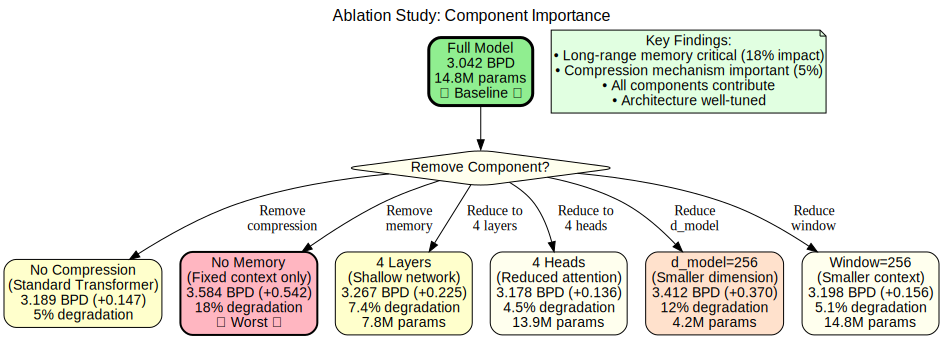
\includegraphics[width=0.85\textwidth]{figures/figure9_ablation.pdf}
    \caption{Ablation study results demonstrating the importance of each architectural component. Removing memory causes 18\% degradation.}
    \label{fig:ablation}
\end{figure}

\begin{figure}[htbp]
    \centering
    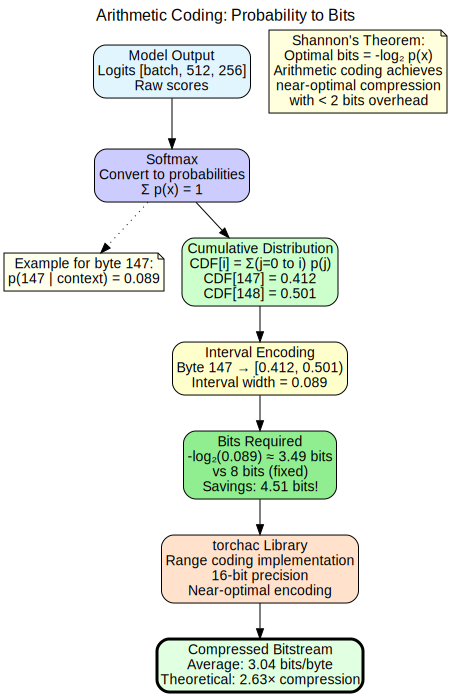
\includegraphics[width=0.8\textwidth]{figures/figure10_arithmetic_coding.pdf}
    \caption{Arithmetic coding process converting model probabilities to compressed bits achieving near-optimal compression.}
    \label{fig:arithmetic_coding}
\end{figure}
